\DiaryEntry{Certain Nonlinear Diophantine Equations}{2023-03-28}{Number Theory}

Coming from \cite{Burton2011}, chapter 12.

\subsection{The Equation $x^2 + y^2 = z^2$}

We first consider the equation

\bee
x^2 + y^2 = z^2
\eee

Because the length $z$ of the hypotenuse of a right triangle is related to the lengths $x$ and $y$ of the sides by the famous Pythagorean equation $x^2 + y^2 = z^2$, the search for all positive integers that satisfy  is equivalent to the problem of finding all right triangles with sides of integral length.

A set of integers $(x,y,z)$ is called a \emph{Pythagorean triple} if $x^2 + y^2 = z^2$ and the triple is said to be primitive if $\gcd(x,y,z) = 1$.

Well-known examples of primitive Pythagorean triples are $(3,4,5), (5, 12, 13)$, and $(12, 35, 37)$.

Suppose that $(x,y,z)$ is any Pythagorean triple and $d = \gcd(x,y,z)$. We therefore can write $x = d x_1, y = d y_1, z = d z_1$ with $\gcd(x_1, y_1, z_1) = 1$ and then we have

\bee
x_1^2 + y_1^2 = \frac{x^2 + y^2}{d^2} = \frac{z^2}{d^2} = z_1^2
\eee

so ($x_1, y_1, z_1)$ is a primitive Pythagorean triple. Thus, it is enough to occupy ourselves with finding all primitive Pythagorean triples; any Pythagorean triple can be obtained from a primitive one upon multiplying by a suitable nonzero integer.

We have two more facts about Pythagorean triples.

\begin{theorem}\label{2023-03-28:th1}
If $(x, y, z)$ is a primitive Pythagorean triple, then one of the integers $x$ or $y$ is even, while the other is odd.
\end{theorem}

Proof: If $x$ and $y$ are both even, then $2|x, 2|y$, and $2 | (x^2+y^2)$ or $2|z^2$ from which follows $2|z$. Therefore, $\gcd(x,y,z) \geq 2$, which contradics the assumption that $(x,y,z)$ is is a primitive Pythagorean triple. If both $x$ and $y$ were odd, then $x^2 \equiv 1 \mod 4$ and $y^2 \equiv 1 \mod 4$ (just try it odd for odd $x$), leading to

\bee
z^2 = x^2 + y^2 \equiv 1 \mod 4
\eee

But this is equally impossible, because the square of any integer must be congruent either to $0$ or to $1$ modulo $4$.\qed

In the following, we will choose $x$ to be even and $y$ to be odd. Then $x^2$ is even, $y^2$ is odd. Therefore $z^2$ is odd, and $z$ is odd as well. We can choose even/oddness differently, but exactely one will be even, while the other two will be odd.

By virtue of above theorem, there exist no primitive Pythagorean triple $(x , y, z)$ all of whose values are prime numbers (as one number is even). There are primitive Pythagorean triples in which $z$ and one of $x$ or $y$ is a prime; for instance, $(3, 4, 5)$, $(11, 60, 61), (19, 180, 181)$. It is unknown whether there exist infinitely many such triples.

We have another theorem about when numbers are powers.

\begin{theorem}\label{2023-03-28:th2}
If $ab = c^n$, with $\gcd(a,b) = 1$, then $a$ and $b$ are $n$-th powers; i.e. $a=a_1^n$ and $b = b_1^n$.
\end{theorem}

We assume $a,b > 1$ and write down the prime factorization of $a$ and $b$ as

\bee
a = p_1^{k_1} p_2^{k_2} \cdots p_r^{k_r}, \quad b = q_1^{j_1} q_2^{j_2} \cdots q_s^{j_s}
\eee

Because $\gcd(ab) = 1$, no $p_i$ can occur among the $q_i$ and therefore the prime factorization of $ab$ is

\bee
ab  = p_1^{k_1} p_2^{k_2} \cdot p_r^{k_r} q_1^{j_1} q_2^{j_2} \cdots q_s^{j_s}
\eee

Let's suppose that the prime factorization of $c$ is equal to $c = u_1^{l_1} u_2^{l_2} \cdots u_t^{l_t}$ and then $ab = c^n$ becomes

\bee
p_1^{k_1} p_2^{k_2} \cdot p_r^{k_r} q_1^{j_1} q_2^{j_2} \cdots q_s^{j_s} = u_1^{n l_1} u_2^{n l_2} \cdots u_t^{n l_t}
\eee

From this we see that the primes $u_1, \ldots, u_t$ are the $p_1, \ldots,p_r, q_1, \ldots, q_s$ in some order and the $n l_1, \ldots, n l_t$ are the corresponding exponents $k-1, \ldots, k_r, j_1, \ldots, j_s$ (again in some order). From this we conclude that the $k_i$ and $j_i$ must be divisible by $n$. We therefore can define $a_1$ and $b_1$ as

\bee
a_1 = p_1^{k_1 / n} p_2^{k_2 / n} \cdots p_r^{k_r / n}, \quad b_1 = q_1^{j_1 / n} q_2^{j_2 / n} \cdots q_s^{j_s / n}
\eee

and therefore $a_1^n = a, b_1^n = b$. \qed

As a simple example, we have $6^2 = 36 = 4 \cdot 9$. The two factors are relatively prime and therefore they must be powers, $4 = ^2, 9 = 3^2$. Note that this $\gcd$ condition depends on the factorization; e.g. $12^2 = 144 = 16 \cdot 9 = 8 \cdot 18$. The first factorization has relatively prime factors, $\gcd(16, 9) = 1$, and correspondingly, we can express the factors as sqaures, $16 = 4^2, 9 = 3^2$. The second factorization is not relatively prime, $\gcd(8, 18) = 2$, and neither is a square.


With all this in place, we can characterize all primitive Pythagorean triples as follows.

\begin{theorem}\label{2023-03-28:th3}
All the solutions to the Pythagorean equation

\bee
x^2 + y^2 = z^2
\eee

satisfying the conditions

\bee
\gcd(x,y,z) = 1, \quad 2 | x, \quad x,y,z > 0
\eee

are given by the formulas

\bee
x = 2st, \quad y = s^2-t^2, \quad z = s^2 + t^2
\eee

for integers $s > t > 0, \gcd(s,t)=1$, and $s \not\equiv t \mod 2$.
\end{theorem}

Proof: Assume that $(x,y,z)$ is a primitive Pythagorean triple. We have chosen $x$ to be even, and $y,z,$ as odd. Therefore $z-y$ and $z+y$ are even; define $z-y=2u$ and $z+y=2v$. Let's rewrite $x^2+y^2=z^2$ as

\bee
x^2 = z^2 - y^2 = (z-y)(z+y)
\eee

and therefore

\bee
\left( \frac{x}{2} \right)^2 = \left( \frac{z-y}{2} \right) \left( \frac{z+y}{2} \right)^2 = uv
\eee

We notice that $u$ and $v$ are relatively prime; if $\gcd(u,v) = d > 1$, then $d | (u-v)$ and $d | (u+v)$, or $d|y$ and $d|z$, which violates the fact that $\gcd(y,z)=1$. Using the previous theorem, we can express $u, v$ as

\bee
u=t^2, \quad v = s^2
\eee

where $s$ and $t$ are positive integers. Substituting everything back yields

\begin{align*}
z &= u + v = s^2 + t^2 \\
y &= v - u = s^2 - t^2 \\
x^2 &= 4uv = 4s^2t^2 \rightarrow x = 2st
\end{align*}

A common factor of $s$ and $t$ would also divide both $y$ and $z$; the condition $\gcd(y,z) = 1$ forces $\gcd(s,t) = 1$. Finally, we observe that if $s$ and $t$ were both even or both odd, then this would make both $y$ and $z$ even which is not possible. Hence, one of the pair $s,t$ is even, the oher is odd - this can also be written as $s \not\equiv t \mod 2$.

In the other direction, we take $x = 2st, y = s^2-t^2, z = s^2 + t^2$ and check that

\bee
x^2 + y^2 = (2st)^2 + (s^2-t^2)^2 = (s^2 + t^2)^2 = z^2
\eee

To see that this triple is primitive, we assume that $\gcd(x,y,z) = d > 1$ and take $p$ to be any prime divisor of $d$. We must have $p \neq 2$ because $p$ divides the odd integer $z$ (one of $s$ and $t$ is odd, the other even, and therefore $z = s^2 + t^2$ must be odd). From $p | y$ and $p|z$, we obtain $p | (z+y)$ and $p | (z-y)$. From the definitions $y = s^2-t^2, z = s^2 + t^2$ follow $z+y=2s^2$ and $z-y=2t^2$ and therefore $p|2s^2$ and $p|2t^2$. But then $p|s$ and $p|t$ and this is incompatible with $\gcd(s,t)=1$. To resolve this contradiction, we must have $d=1$ and $(x,y,z)$ contitutes a primitive Pythagorean triple. \qed

The following screenshot shows a table with some Pythagorean triples. For each value of $s$, we have taken those values of $t$ that are relatively prime to $s$, less than $s$, and even whenever $s$ is odd.

\begin{figure}[H]
    \centering
    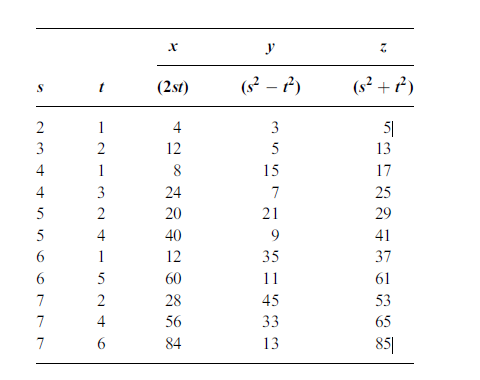
\includegraphics[scale=0.75]{images/2023-03-28-triples.png}
\end{figure}

Looking at this, we suspect that if $(x , y, z)$ is a primitive Pythagorean triple, then exactly one of the integers $x$ or $y$ is divisible by $3$. According to the previous theorem, we have $x=st, y=s^2-t^2, z=s^2+t^2$ with $\gcd(s,t)=1$, If either $3|s$ or $3|t$, then $3|x$ and we are done. Now consider the case that $3 \nmid s$ and $3 \nmid t$. That is, we can write $s = 3k+1$ or $s=3k+2$. In the first case, $s^2 =  9k^2 + 6k + 1 \equiv 1 \mod 3$; in the latter case, $s^2 = 9k^2 + 12k + 4 \equiv 1 \mod 3$. Therefore, $y = s^2 - t^2 \equiv 0 \mod 3$. So, $y$ is divisible by $3$. \qed

The following Figure shows the distribution of primitive Pythagorean triples for values $x, y < 2500$.

\begin{figure}[H]
    \centering
    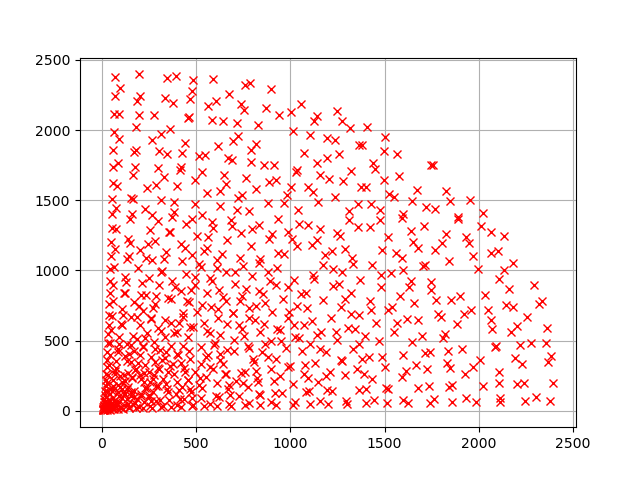
\includegraphics[scale=0.75]{images/2023-03-28-triples_2.png}
\end{figure}


\paragraph{Problem 12.1} a) Find Pythagorean triples (not necessarily primitive) of the form $(16,y,z)$.

We start by $x= 2st$ from Theorem \ref{2023-03-28:th3} from which we obtain $st = 8$. The easiest way is to enumerate all $(s,t)$; however, we have to keep in mind that $s > t > 0$ and $\gcd(s,t) = 1$. There are not many left, in fact only the pair $(s=8, t=1)$. From this follows $y = s^2 - t^2 = 63$ and $z = s^2 + t^2 = 65$ and our first primitive triple is $(16, 63, 65)$. Since there are no other $(s,t)$ combinations possible, we have to find non-primitive Pythagorean triples and multiply them with some factor to obtain a triple of the desired form $(16, y, z)$.

Let's start with triples of the form $(2, y, z)$: We have $2st = 2 \rightarrow st = 1$ but conditions $s > t > 0$ and $\gcd(s,t) = 1$ forbid any solution. Let's consider $(4, y, z)$ instead: $2st = 4 \rightarrow st = 2$ and this is only fulfilled by $s = 2, t=1$. From this follows the triple $(4,3,5)$. Now we multiply with $4$ and obtain the non-trivial triple $(16, 12, 20)$. Another triple can be found based on the primitive triple $(8, y, z)$. Here, $st=4 \rightarrow s = 4, t=1$, and we obtain $(8, 15, 17)$ which becomes $(16, 30, 34)$ by multiplication with $2$. \qed

The b) part is finding primitive Pythagorean triples of the form $(40,y,z)$ and $(60,y,z)$. Nothing fancy to be seen here; basically, we have $2st = 40$, then we list all valid $(s,t)$ combinations and calculate $y$ and $z$ of these (like done above) - that's it.

\paragraph{Problem 6} Show that $(3,4,5)$ is the only primitive Pythagorean triple involving consecutive positive integers. We can write this down as

\bee
x^2 + (x+1)^2 = (x+2)^2 \rightarrow x^2 - 2x - 3 = 0
\eee

and we can solve this quadratic equation as

\bee
x_{1,2} = 1 \pm \sqrt{1+3} = 1 \pm 2 = \begin{cases} &3 \\ &-1 \end{cases}
\eee

Only the positive solution makes sense and this is exactely $(3,4,5)$. Multiplying this triple by some number $k$ yields a non-primitive Pythagorean triple and this won't have consecutive integers; e.g. $(6, 8, 10)$, so $(3,4,5)$ is the only one.

\paragraph{Problem 9} a) Prove that if $(x , y, z)$ is a primitive Pythagorean triple in which $x$ and $z$ are consecutive positive integers, then

\bee
x = 2t(t+1), \quad y = 2t+1 \quad z = 2t(t+1)+1
\eee

for some $t > 0$. We start by noting that $z - x = 1 = s^2+t^2 - 2st = (s-t)^2$ from which follows $s - t = 1$ or $s = t+1$. Inserting this into $x = 2st$ yields $x = 2t(t+1)$ and $y = s^2-t^2 = (t+1)^2 - t^2 = 2t+1$. Finally, $z = x+1 = st(t+1)+1$. \qed

For $t=1$, this yields $(3,4,5)$, for $t=2$ we obtain $(12, 5, 13)$.

b) Prove that if $(x , y, z)$ is a primitive Pythagorean triple in which the difference $z-y = 2$, then

\bee
x = 2t, \quad y = t^2-1, \quad z = t^2+1
\eee

for some $t > 1$. From $z - y = 2 = s^2+t^2 - (s^2 - t^2) = 2t^2$ we have $t = 1$. So $x = 2st = 2s, y = s^2-t^2 = s^2-1, z = s^2 + t^2 = s^2 + 1$. \qed

For $s=2$ this yields our well-known $(3,4,5)$, for $s=3$ we obtain $(6,8,10)$, but this is \emph{not} a Pythagorean triple. Be careful - the statement works in the direction "Pythagorean triple" $\rightarrow$ "express $x,y,z$ as ... and \emph{not the other way round}. For $s=4$ the formulas give a Pythagorean triple, $(8, 15, 17)$.

\paragraph{Further Properties.} Wikipedia holds some more interesting stuff. The expression

\bee
\frac{1}{2}(z-x)(z-y) = \frac{1}{2}(s^2+t^2 - 2st)(s^2+t^2-(s^2-t^2) = \frac{1}{2} (s-t)^2 2t^2 = t^2(s-t)^2
\eee

is a perfect square. Note that this is only a necessary condition not a sufficient one (i.e. a triple fulfilling the condition need not be a Pythagorean triple). In addition, from above we see that $(z-x) = (s-t)^2$ is a perfect square as is $\frac{1}{2}(z-y) = t^2$.

\todo{TBC...}


\subsection{Fermat's Last Theorem}

Fermat's last theorem stated that the equation

\bee
x^n + y^n = z^n
\eee

has no solution in the integers for $n > 2$. He stated, "It is impossible to write a cube as a sum of two cubes, a fourth power as a sum of two fourth powers, and, in general, any power beyond the second as a sum of two similar powers. For this, I have discovered a truly wonderful proof, but the margin is too small to contain it."

For $n=4$, there is a proof for this. Let's start with a similar result.

\begin{theorem}
    The Diophantine equation $x^4 + y^4 = z^2$ has no solution in the positive integers $(x,y,z)$.
\end{theorem}

Proof: Let's assume that there exists a solution $(x_0, y_0, z_0)$ of $x_0^4 + y_0^4 = z_0^2$ with $\gcd(x_0, y_0) = 1$ (if $\gcd(x_0, y_0) = d$ we could define $x_0 = d x_1, y_0 = d y_1, z_0 = d^2 z_0^2$ so that $x_1^4 + y_1^4 = z_1^2$ with $\gcd(x_1, y_1) = 1$).

We now rewrite the equation with the new variables,

\bee
(x_0^2)^2 + (y_0^2)^2 = z_0^2
\eee

and from this we see that $(x_0^2, y_0^2, z_0)$ meet the requirements of a Pythagorean triple and we can reuse the stuff the previous Section. In particular, theorem \ref{2023-03-28:th3} states that one of $x_0^2, y_0^2$ is even while the other is odd. Assume that $x_0^2$ (and therefore $x_0$) is even, there exist relatively prime integers $s > t > 0$ satisfying

\bee
x_0^2 = 2st, \quad y_0^2 = s^2 - t^2, \quad z_0 = s^2 + t^2
\eee

where one of $s, t$ is even. If it happens that $s$ is even, then we have

\bee
1 \equiv y_0^2 = s^2 - t^2 \equiv 0 - 1 \equiv 3 \mod 4
\eee

which is not possible. It's a bit tricky to derive this, so here we go a bit more slowly: Above we assumed that $y_0^2$ is odd (and $x_0^2$ is even). Therefore, $y_0$ is also odd and we can write $y_0 = 2k+1$. Squaring this yields $y_0^2 = 4k^2 + 4k + 1 \equiv 1 \mod 4$. Next, we assumed $s$ even, so $s = 2k$, $s^2 = 4k^2 \equiv 0 \mod 4$. Finally, $t$ is odd, and with the same argument as for $y_0^2$, we have $t^2 \equiv 1 \mod 4$. Combining this, we have $s^2 - t^2 \equiv 0 - 1 \equiv 3 \mod 4$.

From this we see that $s$ cannot be even but must be odd and that $t$ is the even integer. So we can write $t = 2r$ and $x_0^2 = 2st$ becomes $x_0^2 = 4sr$ which we can rewrite as

\bee
\left( \frac{x_0}{2} \right)^2 = sr
\eee

Above we noted that $\gcd(s, t) = 1$ and therefore $\gcd(s, r) = 1$ as well. Theorem \ref{2023-03-28:th2} for $n=2$ states that if $ab=c^2$ with $\gcd(a,b)=1$, then $a, b$ are squares as well. In our case, we therefore have that $s, r$ are squares,

\bee
s = z_1^2, \quad r = w_1^2
\eee

for positive integers $w_1, z_1$.

Next, let's apply Theorem \ref{2023-03-28:th3} to $y_0^2 = s^2 - t^2 \rightarrow y_0^2 + t^2 = s^2$. Because $\gcd(s,t) = 1$, we have $\gcd(t, y_0, s) = 1$, thereby making $(t, y_0, s)$ a primitive Pythagorean triple. With $t$ even, we have

\bee
t = 2uv, \quad y_0 = u^2 - v^2, \quad s = u^2 + v^2
\eee

for relatively prime integers $u > v > 0$. The first relation can be rewritten as

\bee
uv = \frac{t}{2}
\eee

and with the definition of $t = 2r$ we have 

\bee
uv = r = w_1^2
\eee

Again using Theorem \ref{2023-03-28:th2}, we see that $u, v$ are both squares, $u=x_1^2, v = y_1^2$ and when we substitute this back into $s = u^2 + v^2$, we obtain

\bee
z_1^2 = s = u^2 + v^2 = x_1^4 + y_1^4
\eee

With $z_1$ and $t$ being positive, we can construct the following relation

\bee
0 < z_1 \leq z_1^2  = s \leq s^2 \leq s^2 + t^2 = z_0
\eee

What we have done is the following: We started with a solution $(x_0, y_0, z_0)$ to $x_0^4 + y_0^4 = z_0^2$ and constructed a solution $x_1, y_1, z_1$ to $x_1^4 + y_1^4 = z_1^2$ with $0 < z_1 < z_0$. We can continue the procedure from above again and again to generate a sequence of solutions with a decreasing sequence of $z$: $z_0 > z_1 > z_2 > \cdots > 0$. But $z$ has to be a positive integer and therefore this procedure will eventually run into a contradiction. We therefore conclude that $x^4 + y^4 = z^2$ has no solution in the positive integers. \qed

As a consequence, we immediately have the following theorem.

\begin{theorem}
    The equation $x^4 + y^4 = z^2$ has no solution in the positive integers.
\end{theorem}

Proof: If $x_0, y_0, z_0$ were a positive solution of $x^4 + y^4 = z^4$, then $(x_0, y_0, z_0^2)$ would satisfy $x^4 + y^4 =z^2$ which is not possible as just shown. \qed

If $n > 2$, then $n$ is either a power of $2$ or divisible by an odd prime $p$. In the first case, $n =4k$ for some $k \geq 1$ and $x^n + y^n = z^n$ can be rewritten as

\bee
(x^k)^4 + (y^k)^4 = (z^k)^4
\eee

But we have just seen that this equation has no solution in the positive integers. When $n$ is divisible by an odd prime $p$, then $n = pk$ and we obtain

\bee
(x^k)^p + (y^k)^p = (z^k)^p
\eee

If it could be shown that the equation $u^p + v^p = w^p$ has no solution, then, in particular, there would be no solution of the form $u = x^k, v = y^k, w = z^k$; hence, $x^n + y^n = z^n$ would not be solvable. Therefore, Fermat’s conjecture reduces to this: For no odd prime $p$ does the equation 

\bee
x^p + y^p = z^p
\eee

admit a solution in the positive integers. Fermat's conjecture was unproven for more than 300 years; only in 1994, it was proven by Andrew Wiles.


Let's move on to another closely related Diophantine equation, $x^4 - y^4 = z^2$ whcih is also unsolvable.

\begin{theorem}\label{2023-03-28:th4}
The Diophantine equation $x^4 - y^4 = z^2$ has no solution in the positive integers $x, y, z$.
\end{theorem}

Proof: Similar to before, we provide via contradiction. Assume we have a solution $x_0, y_0, z_0$ in the positive integers with a least value $x$. Then $x_0$ has to be odd \todo{why}. Were $\gcd(x_0, y_0) = d > 1$, then defining $x_0 = d x_1, y_0 = d y_1$, we would have $d^4(x_1^4 - y_1^4) = z_0^2$ which would result in $d^2 | z_0$or $z_0 = d^2 z_1$ for some $z_1 > 0$. So $x_1, y_1, z_1$ would be another solution to the equation with $0 < x_1 < x_0$ which is a contradiction. So, we can stick to a solution $x_0, y_0, z_0$ with $\gcd(x_0, y_0) = 1$.

The following argument depends on whether $y_0$ is even or odd.

We start with $y_0$ being an odd integer. We rewrite the equation as

\bee
z_0^2 + (y_0^2)^2 = (x_0^2)^2
\eee

and we see that $(z_0, y_0^2, x_0^2)$ is a Pythagorean triple. Therefore, we can express the solution by means of two relatively prime integers $s, t$ with $s > t > 0$ as

\bee
z_0 = 2st, \quad y_0^2 = s^2 - t^2, \quad x_0^2 = s^2 + t^2
\eee

This ensures the assumned oddness of $y_0$. Multiplying the last two equations together, we arrive at

\bee
x_0^2 y_0^2 = (x_0 y_0)^2 = (s^2 - t^2)(s^2 + t^2) = s^4 - t^4
\eee

Therefore, the triple $s, t, x_0 y_0$ is a solution to $x^4 - y^4 = z^2$. But we have

\bee
0 < s < \sqrt{s^2 + t^2} = x_0
\eee

and this contradicts the assumption that $x_0$ is the minimal solution.

Next we assume that $y_0$ is even. We still have that $(z_0, y_0^2, x_0^2)$ is a Pythagorean triple; since $y_0$ is even, we have

\bee
y_0^2 = 2st, \quad z_0 = s^2 - t^2, \quad, x_0^2 = s^2 + t^2
\eee

We chose $s$ to be even and $t$ as odd and therefore $\gcd(2s, t) = 1$. Since $y_0^2 = (2s)t$, we can apply \ref{2023-03-28:th2} and we can write $2s$ and $t$ as squares of integers: $2s = w^2, t = v^2$. Therefore $w$ has to be even, $w = 2u$ and $s = w^2 / 2 = 2u^2$. We have

\bee
x_0^2 = s^2 + t^2 = 4u^4 + v^4
\eee

and so $(2u^2, v^2, x_0)$ form a primitive Pythagorean triple which we can express as

\bee
2u^2 = 2ab, \quad v^2 = a^2 - b^2, \quad x_0 = a^2 + b^2
\eee

with $\gcd(a,b) = 1$. From $u^2 = ab$ follows that we express $a, b$ as perfect sqaures again, $a = c^2, b = d^2$. Substituting back we obtain $v^2 = c^4 - d^4$ and so we have found another solution to $x^4 - y^4 = z^2$ with the property that

\bee
0 < c = \sqrt{a} < a^2 + b^2 = x_0^2
\eee

This, however, contradicts the initial assumption that $x_0$ is the solution with the smallest value of $x$.

The conclusion of all this is that $x^4 - y^4 = z^2$ has no solution in the positive integers. \qed

Last but not least we find the following.

\begin{theorem}
The area of a Pythagorean triangle can never be equal to a perfect (integral) square.
\end{theorem}

Proof: Consider a Pythagorean triangle with sides $x, y$ and hypotenuse $z$ so that $x^2 + y^2 = z^2$. Its area is $1/2 xy$ and if this were a square, $1/2 xy = u^2$, we would have $2xy = 4u^2$. We can add / subtract this from $x^2 + y^2 = z^2$ to obtain,

\bee
x^2+y^2+2xy = z^2+4u^2 \rightarrow (x+y)^2 = z^2 + 4u^2
\eee

and

\bee
x^2+y^2-2xy = z^2-4u^2 \rightarrow (x-y)^2 = z^2 - 4u^2
\eee

When we multiply these two equations together, we obtain

\bee
(x+y)^2 (x-y)^2 = ((x+y)(x-y))^2 = (x^2-y^2)^2 = (z^2 + 4u^2)(z^2 - 4u^2) = z^4 - 16u^4 = z^4 - (2u)^4
\eee

But this is something of the form $x^4 - y^4 = z^2$ and from Theorem \ref{2023-03-28:th4} we know that this has no solution. Therefore, there can be no Pythagorean
triangle whose area is a square. \qed



%%% Local Variables:
%%% mode: latex
%%% TeX-master: "journal"
%%% End:
